\chapter*{Introduction}
\addcontentsline{toc}{chapter}{Introduction}

\chapter{Problem statement and related work}
In this chapter we introduce the reader to the problematics of genomes comparison. 
We discuss biological relevance of this problem and it's theoretical and technical challenges. 
We finish with an overview of related work.

\section{Biological motivation}

Deoxyribonucleic acid (\textbf{DNA}) is a molecule that caries genetic information of a cell, 
determining it's growth, development, functioning and reproduction. 
DNA molecules are organized in two facing strands which are composed of simpler monomer units called nucleotides.
Each nucleotide is composed of one of four nitrogen-containing nucleobases—either cytosine (C), guanine (G), adenine (A), or thymine (T).
The bases of the two separate strands are bound together according to base pairing rules (A with T, and C with G) to form double-stranded DNA. 

Natural representation of a genome is a sequence/string of letters A, C, T, G corresponding to four bases. 
Note that thanks to the pairing rule we can store the genome as only the sequence for a single strand. 
The usual length of these strings is between $10^6$ and $10^{10}$
of characters.

It is convenient to tell a difference between multiple genome sequences. 
We can ask about simple characteristics like number of C bases and compare those characteristics across multiple genomes. 
Moreover we can ask about specific small sequences that were changed. Note figure X where we can see an absence of a sequence <placeholder> in <placeholder> genome.  

TODO real world example REDO!!!

These specific differences are called variants.
Variants are responsible for differences in individuals.
If we know the difference between two individuals, we can determine the variant that is responsible for this difference. 
Vice versa by detecting a variant in two genomes we, can determine otherwise undetectable difference.
So if we know a variant between cell with cancer and healthy cell we can try to find this variant in different cells and determine, if they started to mutate dangerously.

\section{Genome sequencing}

Determining the genome sequence for a physical DNA is done by DNA sequencing. 
Currently most used sequencing techniques cannot read the whole sequence at once,
instead they produce set of short, overlapping substrings of sequence called reads. 
These techniques also provide a measure of read quality, that is how certain we could be about a given base.
It is assumed that locations of these substrings are sampled uniformly across the original string.
Collection of reads for a given genome is called library.

Other important form of sequencing data are paired reads. 
Paired reads are two reads, for which we know their approximate distance in the genome. 
The total reads length plus the approximated distance is referred to as insert size.

The most important read characteristics are number of errors and length of reads. 
Various read characteristics are determined by used DNA sequencing method.
Note that there is a lot of other attributes that are very important for practical sequencing.
These attributes are throughput, reads, runtime, instrument cost, resources needed for data post-processing.
They explain some surprisingly high or low costs of some methods.

As current sequencing techniques are rapidly improving, we did a basic overview of currently most popular ones. We only considered their attributes relevant for our problem. 
Our data are based on overview from year $2012$ by Quail\cite{quail2012tale} and Liu\cite{liu2012comparison}, 
and on overview from year $2016$ by Goodwin \cite{goodwin2016coming}. 
The first one is important even if it is outdated, 
because we do not necessary have data sampled with the latest methods.

\begin{table}[h]
\centering
\caption{Overview of sequence technologies for year $2012$}
\label{my-label}
\begin{tabular}{|l||c|c|c|c|}
\hline
Technology & \specialcell[c]{Read \\ length (bp)} & \specialcell[c]{Paired \\ reads }& \specialcell[c]{Error\\ rate (\%)} & \specialcell[c]{Cost per million\\bases (\$)} \\
\hline
\specialcell[l]{454 GS FLX \\Titanium XLR70 }& 700 & Yes & 0.1  &  10 \\
Illumina HiSeq 2000 & 150 & Yes & 0.8 & 502 \\
Illumina GAIIx & 150 & Yes & 0.76 & 148 \\
Illumina MiSeq & 1500 & Yes & 12.86 & 2000\\
Ion Torrent PGM & 200 & Yes & 1.71 & 1000\\
PacBio RS & 1500 & No & 12.86 & 2000\\
Sanger 3730xl & 400-900 & No & 0.001 & 2400\\
SOLiDv4 & 50 & Yes & 0.04 & 0.13\\
\specialcell[l]{Oxford Nanopore \\MK 1 MinION} & 200000 & No & 12 & 750\\
 
\hline
\end{tabular}
\end{table}

This shows, we are going to encounter $150b$ long paired reads with an error rate at around $1\%$.


\section{Genome alignment and assembly}
One common approach to variant detection is to reconstruct the sequence based on reads and then compare reconstructed sequences. 
In some cases, one sequence is already known and it is called reference sequence. 
Methods, that do not rely on the reference sequence are called de novo.

The sequence reconstruction problem is referred to as sequence assembly. 
Common formulation for this problem is as a shortest common superstring problem.
\begin{definicia}[Shortest common supersting] 
Given set of strings $\mathcal{P} = {S_1 , S_2 , . . . , S_k }$,
the shortest common superstring is a shortest string $S$, that contains every string from $\mathcal{P}$ as a substring. 
\end{definicia}

This problem proves to be NP-hard \cite{gallant1980finding}.

Other common formulation is to find string by maximal likelihood. 
\begin{definicia}[Maximum likelihood supersting] 
Given set of strings $\mathcal{P} = {S_1 , S_2 , . . . , S_k }$,
the Maximum likelihood supersting is a string $S$, that maximize probability of observing $\mathcal{P}$ as a substring. 
\end{definicia}

These definitions could be extended to work with paired reads as well.

If we could reliably find the original DNA sequence, we could find variants by aligning those sequences.

Informally, sequence alignment is a way of arranging the sequences to identify regions of similarity. 
Aligned sequences of are typically represented as rows within a matrix. 
Gaps are inserted between the letters so that identical or similar characters are aligned in successive columns.

TODO example variant aligning

Reconstructing the original sequence as defined above is often very hard.
Moreover most of the times the sequence contains a lot of errors, ambiguities and regions of low reliability. 
Sequences also contain so called repeats, sequences that are repeated multiple times, 
which are hard to correctly assembly, but could be very important variants.

In practice there are even more problems like reverse complement, diploid genomes, errors in reads, paired reads.
TODO CITE and REF
These can make the retrieved sequence even more ambiguous.

Most genome assembly algorithms focus only on the most probable assembly. 
However, if want to find the most probable variant, we must consider all possible assemblies. 
This is not feasible in an context of standard assembly and alignment.

\section{Problem statement}

TODO variant specification/definition. This will be added after we will see, what specific variants we can detect and describe.

TODO formal definition. We are not sure if we want to define variants as aWb - aXb \ref{def:variant} or something different.

As seen in chapter above, for the purpose of variant detection it might be better to get rid of the assembly and alignment steps. 

For this problem, some work has been already done \ref{sec:related}.
However proposed methods have a lot of shortcomings.
They lack concrete probabilistic foundation, do not incorporate paired reads or do not consider combinations of reads from different sources.

We would like to overcome as much of thees shortcomings and present de novo probabilistically 
grounded method for variant calling using paired reads and multiple sequencing technologies. 

\section{Related work} \label{sec:related}

\subsection{Bidirected de Bruijn graph}
A common method to represent reads is a de Bruin graph. 
This structure serves as a foundation for many assembly and alignment algorithms. (TODO ref)

It's mutations (TODO ref) are used for variant callings as well.

A de Bruijn graph \cite{de1946combinatorial} is a structure for representing overlaps between strings.

\begin{definicia}[de Bruijn graph]
A de Bruijn graph is directed graph. 
For given $k$, vertices of De Bruijn graph represent sequences of length $k$ ($k$-mers). 
The edges of de Bruijn graph represent possible overlaps of length $k-1$, i. e. if have have an edge $(u, v)$ and vertex $u$ represents $k$-mer $a_1 , a_2 , \ldots , a_k$, 
then vertex $v$ represents $k$-mer $a_2 , a_3 , \ldots , a_k , x$ and $k$-mer in vertex $v$ can follow $k$-mer in vertex $u$.
\end{definicia}

Intuitively an edge $(u, v)$ in de Bruijn graph represents, that $k$-mer $u$ is followed by $k$-mer $v$ in the DNA sequence.

Constructing this graph for set of reads is easy.
For each read from $ S_x \in \mathcal{P}$ we construct a set of all its $k+1$-mers. 
Each of this $k+1$-mers consist of two overlapping $k$-mers $k_1, k_2$, 
hence we can add new vertices $k_1, k_2$ with an edge $(k_1, k_2)$ to the da Bruijn graph.
Note that each edge can be in a graph multiple times. 
This is called coverage, and it represents the number of observations that $k_1$ if followed by $k_2$. 

De Bruijn graphs are widely used in genome assembly and underlie many popular algorithms, including AllPaths-LG, SOAPdenovo, Abyss and Velvet. (TODO refs)
This approach can be extended for comparing two libraries. 
We create one de Bruijn graph out of both of them, but each vertex and each edge will be colored based on the library they are from.

If both libraries are the same, than each node and each vertex has both colors. 

\begin{definicia}[variant] \label{def:variant}
Let $a,w,w^*,b, A, B$ be strings over alphabet $\Sigma$.
Strings $a.w.b$ and $a.w^*.b$ are variants of sequences $A$ and $B$, 
if $A$ contains $a.w.b$ and $B$ contains $a.w^*.b$.
\end{definicia}

If the initial sequences $A$ and $B$ contain variants, 
those variants will show as bubbles\cite{iqbal2012novo} in the resulting de Bruijn graph.

\begin{figure}[h]
    \centering
    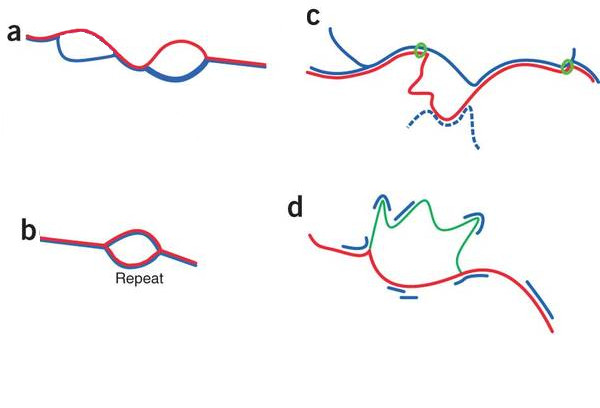
\includegraphics[width=0.5\textwidth]{images/coloreddebruijn}
    \caption{Schematic representation of methods for variation analysis using colored de Bruijn graphs. 
    Coverage is represented by line width.}
    \label{fig:mesh1}
\end{figure}

(TODO draw better pictures)

There is a number of ways to analyze these bubbles.
(a) The simplest $a.w.b$ and $a.w^*.b$ variant is showed as two parts that diverge and merge together forming a bubble.
(b) Repeats also form bubbles, but note that these bubbles have both colors.
(c) When the graph does not form a clean bubble, we can identify variant sites by tracking the divergence of paths.
On finding a breakpoint, we take the longest contig in the sample (that is, the path as far as the next junction) and ask whether the red path returns before this point (green circles show the anchoring sequence).
(d) The likelihood of any given genotype can be calculated from the coverage (blue) of each allele (green, red), accounting for contributions from other parts of the genome. In this example, the sample is heterozygous and therefore has coverage of both alleles, although not sufficient to enable full assembly.

Unfortunately, these approaches do not provide concrete probabilistic justification for used methods. 
Moreover they do not use information about paired reads, which proved to be valuable to decide complicated de Bruijn structures. (TODO cite)
 
(TODO ref cite Computability of Models for Sequence Assembly)

\subsection{Bubble calling}
As each variant corresponds to a bubble, we just need to find all bubbles. 

\begin{definicia}[$(s, t)$ -path]
Given two vertices $s$ and $t$ in $G$, an $(s, t)$-path is a path from $s$ to $t$. 
\end{definicia}

\begin{definicia}[$(s, t)$ -bubble]
is set of two vertex-disjoint $(s,t)$-paths. 
\end{definicia}


\begin{definicia}[$(s, t, \alpha_1, \alpha_2)$-bubble]
in a weighted directed graph is a (s, t)-bubble with paths $p_{1}$ , $p_{2}$ 
satisfying $\| p_{1} \| \leq \alpha_{1}$ and $\| p_{2} \| \leq \alpha_{2}$ .
\end{definicia}

\begin{definicia}[$(s, t, \mathcal{A})-d$-bubble] 
Let $d$ be a natural number and $A = \{\alpha_1 ,\cdot , \alpha_d \} \subset Q_{\geq 0}$. 
Given a directed weighted graph $G$ and two vertices $s$ and $t$, 
a $(s, t, \mathcal{A})- d$ - bubble is a set of $d$ pairwise internally vertex-disjoint paths $\{p_1 , \ldots, p_d \}$, 
satisfying $\|p_i\| \leq \alpha_i \forall i \in [1, d]$.
\end{definicia}

For finding variants we need to solve problem of having a $(s, t, \alpha_1, \alpha_2)$--bubble.
Given a non-negatively weighted directed graph $G$, a vertex $s$,
a set $A = \{\alpha_1 ,\ldots , \alpha_d \} \subset \mathcal(Q)_{\geq 0}$ and $d \in \mathcal{N}$, decide if there exists a $(s, t, \mathcal{A})-d$-bubble in $G$ , for some $t \in V$.
This problem is a generalization of the two disjoint paths problem with a min--max objective function, which is NP-complete. 
(TODO The complexity of finding two disjoint paths with min--max objective function)

The same goes for problem of enumerating all bubbles in a graph.
Sacomoto et al. \cite{sacomoto2013polynomial} showed the first polynomial delay algorithm to enumerate all bubbles with length constraints in a weighted directed graph. 
Complexity of this algorithm in the best theoretical case for general graphs
is O(n(m + n log n)), hence an O(n(m + n log n)) delay algorithm,
where $n$ is the number of vertices in the graph, $m$ the number of edges. 
In the particular case of de Bruijn graphs, the complexity is $O(n(m + n\log \alpha))$ where $\alpha$ is a constant related to the length of the skipped part in an alternative splicing event. 
In practice, an algorithmic solution in $O(nm\log n)$ appears to work better on de Bruijn graphs built from such data. 
Sacamoto implemented the latter, and showed that it is more efficient than previous approaches and outlined that it allows to discover novel long alternative splicing events.

\subsection{Variant Calling}\label{sub:variantcalling}
Heng Li et al \cite{li2008mapping} introduced quality score for mapping short reads to the reference genome.

They then extended this approach for calling variants between the library and a reference genome and implemented it as an MAQ algorithm.

Heng Li's work was based on finding the best read alignments to the reference sequence. 
He discussed use of Eland-like (A.J. Cox, unpubl.) hashing technique and it's probabilistic interpretation.
Note that this was a probabilistic interpretation of the hashing, not of sequencing.
This hashing is used to find the $28bp$ long beginning (seed) of the read in the reference sequence with some number of acceptable errors.


MAQ then assigns each individual alignment a mapping quality. 
The mapping quality $Q_s$ is the scaled probability (TODO Ewing and Green 1998) that a read alignment may be wrong. 
$$Q_s=-10\log_{10}\Pr(read~is~wrongly~mapped)$$
For example, $Q_s = 30$ implies there is a $1$ in $1000$ probability that the read is incorrectly mapped. 

Heng Li considers a simplistic case where all reads are known to come from the reference and an ungapped exhaustive alignment is performed.
Practical model for alignment with heuristic algorithms is also considered.

They computed the probability $\Pr(z|x,u)$ of read sequence $z$ coming from the position $u$ at the reference sequence $x$, 
on the assumption that sequencing errors are independent at different sites of the read.

To calculate the posterior probability $\Pr_s(u|x,z)$, Heng assumes an uniform prior distribution $p(u|x)$, and applying the Bayesian formula gives 
$P_s(u|x,z)=\frac{P(z|x,u}{\sum_{v=1}^{L-l+1}P(z|x,v)}$ 
where $L = \|x\|$ is the length of $x$ and $l = \|z\|$. 

In practice, Heng approximates $Q_s$ as 
$$Q_s=\min\{q_2 - q_1 - 4.343 \log(n_2), 4+(3-k^*)(\hat{q} -14)-4.343 \log(P_1 (3-k^*, 28) \}$$

Where $q_1$ is the sum of quality values of mismatches of the best read alignment, $q_2$ is the corresponding sum for the second best alignment, 
$n_2$ is the number of alignments having the same number of mismatches as the second best alignment, 
$k$ is the minimum number of mismatches in the $28-bp$ seed, $q$ is the average base quality in the $28-bp$ seed, 
$4.343$ is $\frac{10}{log(10)}$, and $P_1(k,28)$ is the probability that a perfect alignment and a $k$-mismatch alignment coexists given a $28-bp$ sequence that can be estimated during alignment. 

\subsection{Probabilistic model for sequence assembly}

As our problem is closely related to modeling the initial genome, we will base our theory on this modeling.

Several probabilistic models were introduced\cite{rahman2013cgal}\cite{ghodsi2013novo} as a measure of the assembly quality. 
In our work we  will build on those, as there is an clear parallel between assembly quality and
variant quality.
As authors have shown, the likelihood based metrics consistently favors higher quality assemblies, so they should favor higher quality variants as well. 

The probabilistic model defines the probability $\Pr(L|A)$ that a library of sequencing reads $L$ is observed assuming that assembly $A$ is the correct assembly of the genome. 

This model only evaluates quality of a single assembly. 
Boža\cite{bovza2015gaml} extended this model and used it as an optimization criterion in the own process of finding high likelihood genome assemblies.

The model assumes that individual reads are independently sampled, and thus the overall likelihood is the product of likelihoods of the reads: $$\Pr(R|A) = \prod _{r\in R} \Pr (r|A)$$
Boža used the log-average probability of a read, what made the resulting value independent of the number of reads in set R.
$$\text{LAP}(A|R) = \frac{1}{|R|}\sum\nolimits_{r\in R} \log \Pr (r|A)$$

Note that maximizing \(\text {LAP}(A|R)\) is equivalent to maximizing \(\Pr (R|A)\).

If the reads were error-free and each position in the genome was sequenced equally likely, 
the probability of observing read $r$ would simply be $\Pr (r|A)= \frac{n_r}{2L}$, 
where $n_r$ is the number of occurrences of the read as a substring of the assembly $A$, 
$L$ is the length of $A$, and thus $2L$ is the length of the two strands combined. 

The probability of a single alignment with $s$ errors (substitutions and indels) and $m$ matching positions is defined as $\frac{R(s,m)}{2L}$, 
where $R(s,m) = \varepsilon ^{s}(1-\varepsilon )^{m}$ and $\varepsilon$ is the sequencing error rate.

Boža noted, that the full dynamic programming is too time consuming, 
and in practice only several best alignments contribute significantly to the overall probability.

They approximate the probability of observing read $r$ with an estimate based on a set $S_r$ of a few best alignments of $r$ to genome $A$, as obtained by one of the standard fast read alignment tools:
$$\Pr (r|A)\approx \frac{\sum _{j\in S_r} R(s_j, m_j)}{2L}$$

$s_j$ is the number of mismatches and indels implied by the $j^{th}$ alignment alignment and $m_j$ is the number of matches in this alignment. 

Boža also incorporated paired reads. 
They assumed that the insert size distribution in a set of reads $R$ can be modeled by the normal distribution with known mean $\mu$ and standard deviation $\sigma$. 
The probability of observing paired reads $r_1$ and $r_2$ can be estimated from the sets of alignments $(S_{r_1})$ and $(S_{r_2})$ as:
$$\begin{aligned} \Pr (r_1, r_2|A) \approx \frac{1}{2L} \displaystyle \sum _{j_1 \in S_{r_1}} \displaystyle \sum _{j_2 \in S_{r_2}} R(s_{j_1}, m_{j_1}) R(s_{j_2}, m_{j_2}) \Pr (d(j_1, j_2)|\mu , \sigma ) \end{aligned}$$
$(d(j_1,j_2))$ is the distance between the two alignments as observed in the assembly 
and $(s_{j_i})$ and $(m_{j_i})$ are numbers of sequencing errors and matches in alignment $j_i$. 

To model a case where reads are from different libraries obtained by different technologies,
they used different model parameters for each set and compute the final score as a weighted combination of log average probabilities for individual read sets $R_1,\dots, R_k$:
$$\begin{aligned} \text {LAP}(A|R_1, \dots , R_k) = w_1 \text {LAP}(A|R_1) + \dots + w_k \text {LAP}(A|R_k). \end{aligned}$$

\subsection{Indexing techniques}
A lot of times in genome sequencing, assembly, or aligning we need to search in a set of reads.
As discussed at section \ref{sub:variantcalling}, we needed to align multiple reads to the reference sequence. 
As we need to tolerate small mismatches, this problem becomes hard.
Various methods based on Blum filters and hashing were proposed (TODO cite).

In fact this problem appears in other fields. 
\begin{definicia}
Given a set $S$ of $d$ dimensional real value vectors $d_1,d_2 \ldots d_n$, 
retrieve set of $k$ most similar vector query vectors $q_1,q_2,\ldots,g_m$.  
\end{definicia}

Similarity is very vaguely defined, because we are often interested in different similarities in different spaces like $L_1$, Levenshtein, euclidean 
or even non-metric ones like KL-divergence, cosine distance or Itakura-Saito.

This problem is called K-nearest neighbor search problem (K-NNS). 
In its approximated version (K-ANNS) we allow some false positive results.

Authors \cite{malkov2012scalable,malkov2014approximate} proposed a proximity graph K-ANNS algorithm called Navigable Small World (NSW), 
which utilized navigable graphs with long range links constructed by a much simpler model. 

Malkov\cite{malkov2016efficient} introduced and implemented\cite{nmslib2016} an algorithm for the K-ANNS based on navigable small world graphs with controllable hierarchy (Hierarchical NSW).

Hierarchical NSW incrementally builds multi-layer structure consisting from hierarchical set of  proximity graphs for nested subsets of the stored elements.
The maximum layer in which an element is present is selected randomly with exponentially decaying  probability distribution.
Starting search from the upper layer together with utilizing the scale separation boosts the performance compared and allows a logarithmic complexity scaling. 

Additional employment of a heuristic for selecting proximity graph neighbors significantly increases performance at high recall and in case of highly clustered data. 
Performance evaluation has demonstrated that the proposed general metric space method is able to strongly outperform many previous state-of-art vector-only approaches. 

Malkov's\cite{malkov2016efficient} algorithm based on idea s close to NSW, very good logarithmic complexity scaling. 
The main contributions were smart selection of the graph’s enter-point node, separation of links by different scales and using a slightly more complicated heuristic to select the neighbors. 

\subsection{A*}
Our algorithm will be probably based on some form of de Bruijn graph traversal. 
Paired reads and long reads provide information about real distance between two nodes in de Bruijn graph.

Incorporating this information in process of graph traversal can be hard. 
We took an inspiration from a well known $A^*$ algorithm.


\chapter{Proposed probabilistic approach 5 pages}
To continue we need a few definitions. Let $v$, $w$ be two strings over alphabet $\Sigma = \{A, C, G, T \}$. Concatenation of these strings is denoted as $v . w$. 

We will extend the de Bruijn definition. TODO extended de Bruijn graph definition


\chapter{Catchy name for our tool that will be implemented}
\section{Implementation problems 8}
\section{Data 1}
write about data generation.
\subsection{Variant simulation 2-3}
Here we closely describe methods used for variant generation, and relevant variant parameters.
\subsection{Read simulation 2-3}
Here we evaluate data for reads and we set our expectations about these data.
\subsection{Paired read simulation 2-3}
write about data sources
Here we evaluate data for paired reads and we set our expectations about these data.
\subsection{Real data 2-3}
\section{Metrics 2-3}
Here we discuss what metrics we want to improve and what is the measure of success for our solution.
\section{Benchmarks}
\subsection{Genome alignments 3-4}
Brief mentions of current genome alignments approaches.
\subsection{Without paired reads 2}
\subsection{With paired reads 2}

\section{Results 12}
\section{Future improvements 5}

\chapter{Discussion 2}
Here we will discuss.



